\documentclass{standalone}
\usepackage{tikz}
\usepackage{ctex,siunitx}
\usepackage{tkz-euclide}
\usepackage{amsmath}
\usetikzlibrary{patterns, calc}
\usetikzlibrary {decorations.pathmorphing, decorations.pathreplacing, decorations.shapes,}
\begin{document}
\small
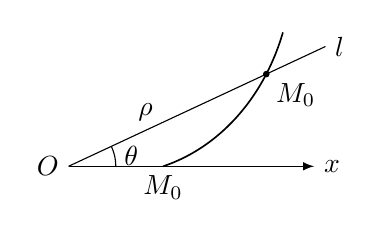
\begin{tikzpicture}[>=latex,scale=1.2]
  \draw [semithick,domain=0:32,samples=200] plot (\x:{1+3*\x/180*pi});
  \draw[->] (0,0)--(2.6,0)node[right]{$x$};
  \draw(25:3)node[right]{$l$}--(0,0)node[pos=0.7,above]{$\rho$};
  \draw(0.5,0)arc(0:25:0.5)node[midway,right]{$\theta$};
  \node at(0,0) [left]{$O$};
  \node at(1,0) [below]{$M_0$};
  \fill (25:5/12*pi+1)circle(1pt)node [below right]{$M_0$};
\end{tikzpicture}
\end{document}